\documentclass[11pt,a4paper]{book}
\usepackage[utf8]{inputenc}
\usepackage[spanish]{babel}
\usepackage{amsmath}
\usepackage{amsfonts}
\usepackage{graphicx}
\usepackage{amssymb}
\usepackage[left=2cm,right=2cm,top=2cm,bottom=2cm]{geometry}
\usepackage{cite}
\usepackage{babelbib}
\usepackage{float}
\author{Víctor de Tejada Molera}

\begin{document}
\chapter{Antecedentes}
    En este capítulo se pretende realizar un análisis del estado del arte referente a los experimentos psicoacústicos; concretamente aquellos que se centran en la evaluación de diferencias perceptuales en entornos cerrados como auditorios, cines, salas de conferencias, etc.
    
    Para la búsqueda de esta información, se recurre a bases de datos científicas como el sistema \textit{Ingenio UPM} y buscadores de artículos científicos como \textit{Google Scholar}. Con ellos, se han introducido términos de búsqueda como ``\textit{Psychoacoustics}'', ``\textit{Subjective test acoustics}'' o ``\textit{Auditorium subjective test}''. Los resultados arrojados por dichas plataformas, se revisan y se lee el resumen o \textit{abstract} de los que se consideran que pueden ser útiles para el proyecto. Si el resumen confirma que la temática concuerda con la del estudio, se procede a la lectura del resto del artículo y se extraen los elementos más importantes. Estos son principalmente: el tipo de análisis estadístico que se ha utilizado, el número de personas que han realizado el test, el tipo de test (tipo de preguntas, formato, duración de los audios utilizados, etc.), entre otros.
    
    Por otro lado, se ha realizado, paralelamente, una búsqueda de fuentes bibliográficas especializados en temas como de detección de señales, análisis estadístico de datos y, más específicamente, sobre modelos Thurstonianos. Para ello, se realizan nuevas consultas a los medios ya presentados a personas con experiencia contrastasda en la realización y el estudio de experimentos psicoacústicos.\newline
    
    Utilizando esta metodología, se han consultado alrededor de 50 documentos entre libros de referencia, normativas internacionales, artículos en revistas y congresos, trabajos de fin de grado, etc. De todo este material, han acabado siendo de utilidad 30 fuentes bibliográficas aproximadamente.
    
    \section{Análisis de la documentación consultada}
    
    Al analizar los distintos documentos, se ha observado una gran inconsistencia en las características de los diferentes estudios que se han analizado. Este problema ya se comenta en algunas fuentes como \cite{Tejada2020}. En este apartado se analizan las características de los proyectos y normativas según varios de sus aspectos más representativos. 
    
        \subsection{Aspectos subjetivos a analizar}
		    Los aspectos subjetivos que se pueden analizar mediante test perceptuales son muy variados. Por un lado algunos experimentos como en \cite{1995GASoulodre, 2016SKlockgether,  2016BPostma, 2002PZahorik} se centran en estudiar las características relacionadas con la reverberación de las salas (persistencia del sonido, diferencias entre sonidos anecoicos y reverberantes, etc.). Otros estudios se centran en el estudio de la inteligibilidad de diferentes señales acústicas \cite{ 1999JBradley, 2010FMartellotta,  2010MVigeant}, mientras otras se centran en temas de localización de sonora \cite{1997SCarlile, 2019MShiell, 2019MYamada, 2019DMorikawa}. También se encuentran aquellos experimentos en los que se pretende estudiar características como las diferencias entre señales, la sonoridad o diferencias de nivel \cite{2019GPulvirenti, 2016SKlockgether, 2019MNowak, 2011VEmiya, 2019LKritly, 2005IWitew,  2019DJSchlit}. Por último, una de las áreas que está teniendo más importancia en los últimos años se corresponden con el estudio de la molestia acústica \cite{2019VHongisto, 2019JLee, 2019VRajala}.
		    
            Algunos documentos como \cite{Tejada2020} tratan de ordenar estas fuentes en diferentes categorías y facilitar el análisis de grandes cantidades de bibliografía y extraer sus elementos comunes.
            
        \subsection{Tipos de test}
    		Por otro lado, se ha observado una gran variedad de formatos para hacer los test. Los más habituales se presentan a continuación.
    
    		\begin{itemize}
        		\item \textbf{Test de diferencias}: En este tipo de test al oyente se le presentan 2 o más audios y tiene que determinar si son iguales o no. Tiene la ventaja de que son sencillos de implementar y de analizar. En algunos sitios, se le llama ``duo'' o ``binomial'' por lo que es importante revisarlos a conciencia para no confundirlos con los ``Duo-Trio'' o un ``ABX''. Algunos de los artículos en los que han aplicado este tipo de test son \cite{1995GASoulodre, 1999JBradley,2002PZahorik, 2005IWitew, 2010MVigeant, 2019LKritly}. Un ejemplo concreto de este tipo de test y que tendrá gran importancia a lo largo del proyecto es el denominado ``2-AFC'' (\textit{Two-Alternative Forced Choice}). En este test, el participante está ``forzado'' a escoger entre dos opciones, no pudiendo seleccionarse una opción intermedia, como respuesta a una pregunta relacionada con su exposición a un determinado estímulo \cite{PsychophysicsB}.
        		\item \textbf{Test Duo-Trio}: Para este formato, se presentan tres audios. Uno de ellos es igual a  uno de los otros dos que se denomina ``Referencia''. El objetivo del oyente es determinar cuál de los audios que se le presenta es igual a dicha referencia. Algunos de los estudios que han utilizado este tipo de test son \cite{delaPrida2019, delaPrida2021}.
        		\item \textbf{ABX}: En este tipo de test se presentan tres señales. El oyente tiene que determinar cuál de las dos primeras que se le presentan es igual a la que es presentada en último lugar. El experimento se repite varias veces modificando la última señal para que no sea siempre el mismo audio. Algunos ejemplos donde se aplican este tipo de test se encuentran en \cite{delaPrida2021, Braun2004}.
        		\item \textbf{Test de escalas numéricas}: El objetivo de este test es que el oyente cuantifique alguna determinada característica de las señales de audio mediante una escala numérica. Algunas variantes permiten que se realice la cuantificación de varios elementos en paralelo o que se pida que se ordenen varios audios simultáneamente en función de la característica que se pretenda evaluar (Test de MUSHRA \cite{UIT1534}). Este tipo de test son muy útiles y aparecen como recomendación por parte de normativas internacionales \cite{UIT1116, UIT1284, UIT1534}.También aparecen en algunos documentos como \cite{2011VEmiya,2016BPostma, 2019ZShao,2019GPulvirenti,2019VRajala, 2019JLee, 2019DMorikawa}. 
        		
    		\end{itemize}
    		Existen otros tipos de test como los triangulares o los A/NotA \cite{delaPrida2021, Brockhoff2009}. No obstante, no se han encontrado experimentos en los que se apliquen dichas metodologías, a parte de ese artículo, por lo que no se han considerado para las siguientes partes del proyecto.
    
    		Cada uno de los tipos de test mencionandos arriba tienen sus propias particularidades, sus ventajas y sus inconvenientes tanto para su realización como para el análisis de sus resultados que se comentarán posteriormente en el capítulo de ``Realización de los test subjetivos de audio''.
    
	    \subsection{Características de los participantes}
    		Si se analizan las características de las personas que participan en los test perceptuales, se observa una gran variedad tanto en el número como en su experiencia. 
    		
    		Por un lado, se tienen estudios que utilizan un número muy pequeño de personas, diez o menos, como es el caso de \cite{2019MNowak, 2002PZahorik, 2016SKlockgether,2019ZShao}. Por otro lado, algunos casos presentan números mucho mayores llegando a utilizar casi cien personas, como ocurre en \cite{1954JEgan}. También se observa que el número de participantes varía en función del aspecto subjetivo que pretenda analizarse \cite{Tejada2020}; de esta forma, los estudios que estudian la molestia acústica son los que utilizan un mayor número de participantes (en torno a los 30-40 según \cite{Tejada2020}), mientras que el resto utilizan unas 20 personas aproximadamente, que se corresponde con las recomendaciones de las normativas \cite{UIT1116, UIT1284, UIT1534}.

            Otro aspecto importante muy relacionado con el número de participantes consiste en la utilización de participantes con o sin experiencia en este tipo de experimentos psicoacústicos. Normativas como \cite{UIT1116, UIT1284, UIT1534} recomiendan la utilización de participantes con experiencia cuando los aspectos a analizar son bastante técnicos o requieren de personas con oídos especializados en la detección de ciertos eventos (como, por ejemplo, educación musical avanzada). No obstante, aceptan la presencia de participantes sin experiencia si se aumenta el número total de personas que participan en el experimento o si se les aplica algún tipo de entrenamiento previo, incluso se recomienda realizarlo para participantes con experiencia.

            A pesar de estas recomendaciones, la realidad es bastante diversa y se encuentran estudios como \cite{1995GASoulodre,1999JBradley, 2005IWitew, 2010FMartellotta, 2010MVigeant, 1997SCarlile, 2011VEmiya, 2016BPostma, 2019ZShao, 2019VRajala, 2019MShiell, 2019JGroose, Braun2004, delaPrida2019, delaPrida2021} en los que sí se aplican entrenamientos previos, mientras que en otros estudios como \cite{Brockhoff2009,2019LKritly,2019DMorikawa, 2019DJSchlit} no se realizan. También se han encontrado varios estudios en los que no se reflejaba si se habían realizado estos entrenamientos o no \cite{2002PZahorik, 2016SKlockgether, 2019GPulvirenti,2019MNowak, 2019MYamada, 2019JLee, Christensen2009}.
    
	    \subsection{Interacción del participante con los estímulos auditivos}
    		A nivel de interacción por parte de la persona participante, existe división de opiniones sobre la posibilidad del usuario de poder controlar la reproducción de los estímulos \cite{1995GASoulodre, 2010FMartellotta, 2010MVigeant, 2011VEmiya,2019DMorikawa} frente a \cite{1999JBradley, 2002PZahorik, 2005IWitew, 2016SKlockgether, 2019VRajala, 2019VHongisto} que no permiten a los participantes esa opción. No obstante, normas como \cite{UIT1116,UIT1534, UIT1284,EBU3286, UIT1285, UIT1286} recomiendan que los participantes tengan, siempre que sea posible, la capacidad de interactuar con los estímulos de forma directa y repetir su reproducción si así lo desean. En ningún momento se hace mención sobre el tiempo máximo que un usuario debe pasar con cada estímulo.
	
        \subsection{Duración del experimento}
    		En cuanto a la duración de los estímulos, se han observado que los valores suelen rondar de 1 a 5 segundos \cite{2010FMartellotta, 2016SKlockgether, 2011VEmiya, 2019LKritly, 2019GPulvirenti, 2002PZahorik, 2019MShiell, 2019JGroose, 2019MNowak, 2019MYamada, 2019DMorikawa, 2019DJSchlit}. No obstante, también se han encontrado estudios donde la duración se encuentra entre los 8-10 segundos \cite{2010FMartellotta, 2019JLee, 2010MVigeant}, obteniéndose casos con un máximo de 15 segundos como en \cite{1995GASoulodre, 2005IWitew}. Esto concuerda con las recomendaciones de \cite{UIT1116,UIT1534, UIT1284,EBU3286, UIT1285, UIT1286} al respecto donde se indica que la duración de dichos estímulos debe ser lo suficientemente reducida para evitar que los participantes se acostumbren a las señales \cite{GelfandStanley}. Unido a esto, la duración total de la sesión, a pesar de ser el apartado del que menos información se aporta, se recomienda que no exceda de los 30 minutos , siendo necesaria la inclusión de descansos de la misma duración, si se tiene que alargar \cite{UIT1116, UIT1284, UIT1534, ZwickerFactsModels, GelfandStanley, BlauertSpatialHearing}. Esto ocurre en casos como \cite{2019LKritly} donde se tiene una duración de casi 90 minutos. En ningún momento se especifica si el entrenamiento previo computa dentro de la duración del experimento, aunque en nuestra experiencia particular, se suele incluir.
    
	    \subsection{Análisis de los datos}
    		En cuanto al análisis de los datos, históricamente se han utilizado procedimientos como los análisis de la varianza (ANOVA) \cite{2011VEmiya, 2016BPostma, 2019LKritly, 2019GPulvirenti, 2019MShiell, 2019VHongisto}, o normas como \cite{ISO10399}. No obstante, en estudios más recientes como \cite{delaPrida2019, delaPrida2021} aparecen los modelos thurstonianos como una alternativa sencilla de aplicar y con cualidades que pueden resultar útiles para ciertos tipos de estudio. Algunos de estos ejemplos se explican con más profundidad en el apartado ``1.2.2 Modelos Thurstonianos''.\newline
    
    A la vista de todo lo expuesto, queda patente la gran variedad de sistemas que se siguen en la actualidad para realizar los test perceptuales. Por ello, para nuestro test es necesario identificar sus particularidades para poder determinar las características que mejor se ajusten al mismo. Esto se trabaja en profundidad en los apartados ``4.1.1 Características del test previo'' y ``4.1.2 Características de los test finales'' siguiendo la metodología del capítulo ``Toma de datos''.
    
    \section{Conceptos teóricos para el análisis estadístico}    
        \subsection{UNE-EN ISO 10399}
            La norma UNE-EN ISO 10399: ``Análisis sensorial. Metodología. Ensayo Duo-Trio.''\cite{ISO10399} es un documento que permite analizar la probabilidad de que eventos perceptuales sean percibidos como iguales o diferentes según el número de respuestas definidas como correctas o erróneas al realizar experimentos basados en test duo-trio. Esta norma no se centra en señales acústicas, sino que puede utilizarse para experimentos subjetivos relacionados con olores, sabores imágnees, etc.
            
        
            Al comienzo del documento se definen diferentes términos que aparecen de forma constante a lo largo de la norma. Para nuestro caso particular, los términos más relevantes son:
        
            \begin{itemize}
                \item alpha-risk o $\alpha$-risk: es la probabilidad, o riesgo, de afirmar que existe una diferencia perceptual cuando en realidad no existe.
                \item beta-risk o $\beta$-risk: es la probabilidad, o riegos, de afirmar que no existe una diferencia perceptual cuando en realidad sí existe.
                \item diferencia perceptual: situación en la que dos o maś muestras pueden ser distinguidas por sus propiedades sensitivas (a través del oído, tacto, gusto, vista, etc.)
                \item similaridad perceptual: situación en la que las diferencias entre muestras son tan pequeñas que no pueden distinguirse entre sí de forma sensitiva.
            \end{itemize}
            Para el cálculo de las probabilidades $\alpha$-risk y $\beta$-risk, la norma proporciona sendas tablas. En este proyecto sólo se precisa el cálculo de $\alpha$ que se encuentran en el Anexo B  (la tabla B.1). También se proporciona la ecuación \ref{eq:alpha} donde se puede calcular el mínimo de respuestas ``correctas'' para que se obtenga un determinado valor de $\alpha$-risk. Con estas herramientas se puede comprobar si los resultados de un test arrojan valores para $\alpha$ y $\beta$ se encuentran dentro de unos determinados valores (20\%, 10\%, 5\%, 1\% y 0.1\%)
            
            \begin{equation}
                x=(n/2)+z*\sqrt{n/4}
                \label{eq:alpha}
            \end{equation}
            
            Donde:
            \begin{itemize}
                \item x: número de respuestas correctas mínimas necesarias para que se obtenga un determinado $\alpha$-risk.
                \item n: número de respuestas totales.
                \item z: variable que toma un valor en función de $\alpha$-risk:
                \begin{itemize}
                    \item 0.84 para $\alpha=0.20$.
                    \item 1.28 para $\alpha=0.10$.
                    \item 1.64 para $\alpha=0.05$.
                    \item 2.33 para $\alpha=0.01$.
                    \item 3.09 para $\alpha=0.001$.
                    
                \end{itemize}
            \end{itemize}
            
            Un ejemplo de aplicación para conocer el coeficiente $\alpha$-risk sería el siguiente: Suponemos que tenemos un caso de estudio entre dos señales acústicas distintas entre sí.  Se ha realizado un test perceptual y se han obtenido 100 respuestas, 87 de las cuales opinan que las dos señales son diferentes.
            
            En primer lugar, se acude a la tabla del Anexo B para comprobar si están los datos para ese número de respuestas. En este caso, se comprueba que, desgraciadamente, la tabla sólo arroja datos hata las 88 respuestas, por lo que se procede a resolver la ecuación \ref{eq:alpha}. Sustituyendo las variables por los datos que se tienen, se obtienen 5 valores diferentes de x para cada uno de los posibles valores de $\alpha$:
            \begin{itemize}
                \item $x=55$ para $\alpha=0.20$.
                \item $x=57$ para $\alpha=0.10$.
                \item $x=59$ para $\alpha=0.05$.
                \item $x=62$ para $\alpha=0.01$.
                \item $x=66$ para $\alpha=0.001$.
            \end{itemize}
            Es importante remarcar que los resultados siempre se redondean hacia arriba, puesto que es imposible tener fracciones de respuestas.
            
            Una vez obtenidos los valores, el valor de $\alpha$ se corresponde con el del caso más cercano que sea inferior a nuestro número de respuestas diferentes. En nuestro caso, $\alpha<0.001$ ya que 66 es el número más cercano a 87 (y además se cumple que es menor).
            
            Como ya se explicó anteriormente, el coeficiente $\alpha$-risk muestra la probabilidad de que dos eventos sean diferentes cuando, en realidad, son iguales. Por este motivo, cuanto más pequeño es el valor del coeficiente, estadísticamente más representativa es la diferencia perceptual. Por este motivo, en estudios como el nuestro, se busca obtener valores pequeños.
            
            Puede ocurrir que se obtengan situaciones donde el número de respuestas en las que se han indicado que son diferentes sea menor que para el caso de $\alpha=0.20$ (en el ejemplo anterior, si se hubiera obtenido menos de 55 respuestas marcadas como diferentes). Si este fuera el caso, no se podría concluir que estadísticamente la percepción de dichos estímulos es diferente. En todo caso, habría que concluir que las posibles diferencias son debidas, mayoritariamente, al azar. 
            
        \subsection{Modelos Thurstonianos}
            Los \textit{modelos Thurstonianos}\footnote{Nombrados así por Louis Leon Thurstone.}\cite{PsychophysicsB, SignalB, delaPrida2019} son modelos estadísticos en los que se utilizan variables de distribuciones normales y que se utilizan en gran medida en estudios de discriminación sensorial. 
            
            En el caso concreto de la psicoacústica, se utilizan generalmente para obtener un valor ``$d'$'' que da información ordenada y cuantitativa sobre una determinada percepción subjetiva. Además de este valor, se calcula a su vez la desviación estandar ``$\sigma$''. Con estos dos valores, se puede aproximar las respuestas de un test subjetivo como una sucesión de distribuciones gaussianas en las que en función del valor ``$d'$''y ``$\sigma$'' están más o menos superpuestas. Esta superposición da información sobre la probabilidad de que ambos estímulos puedan ser distinguibles o no entre sí y cuánto. Esto se observa más fácilmente en la figura \ref{fig:modelost} obtenida en \cite{PsychophysicsB}.
            
            \begin{figure}[H]
                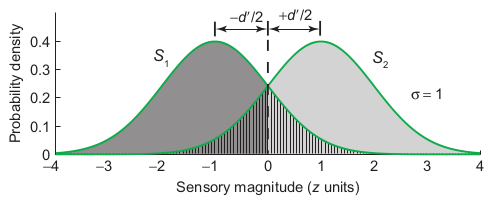
\includegraphics[scale=0.7]{../imagenes/modelosthurst.png}
			    \centering
			    \caption{Ejemplo de cálculo de $d'$ utilizando modelos thurstonianos. Fte: \cite{PsychophysicsB} }
			    \label{fig:modelost}
            \end{figure}
            
            Utilizando la figura \ref{fig:modelost} como ejemplo, se puede suponer que S1 y S2 son las distribuciones obtenidas de las respuestas de un test en las que S1 son las respuestas en las que dos estímulos han sido identificados como iguales, mientras que S2 se corresponde con las respuestas cuando los dos estímulos se identifican como diferentes. Cuanto más se solapen ambas distribuciones, más difícil será para los participantes distinguirlas. Gráficamente resulta fácil comprobar que las variables que determinan este solapamiento es principalemente $d'$, sin dejar de lado la importancia que tiene la desviación estándar $\sigma$.
            
            Además de lo ya expuesto, este tipo de análisis es especialmente interesante porque nos permite ordenar los valores obtenidos para $d'$ de forma que las diferencias entre ellos nos da información cuantitativa sobre cómo de diferentes o de similares son cada una de las distribuciones. Con la facilidad añadida que tiene este sistema para representar gráficamente mediante las técnicas habituales como diagramas de barras, entre otros. También tiene la ventaja de que el valor del coeficiente $d'$ es independiente del tipo de test que se realice, incluso es posible compararlos entre sí \cite{delaPrida2021}.
    
    
    \bibliography{biblio}
    \bibliographystyle{babunsrt}
\end{document}